\documentclass[aspectratio=169]{beamer}
%
% Choose how your presentation looks.
%
% For more themes, color themes and font themes, see:
% http://deic.uab.es/~iblanes/beamer_gallery/index_by_theme.html
%

\setbeamertemplate{itemize/enumerate body begin}{\small}
\mode<presentation>
{
  \usetheme{default} % or try Darmstadt, Madrid, Warsaw, ...
  \usecolortheme{default} % or try albatross, beaver, crane, ...
  \usefonttheme{serif} % or try default, structurebold, ...
  \setbeamertemplate{navigation symbols}{}
  \setbeamertemplate{caption}[numbered]
}
\usepackage[english]{babel}
\usepackage[utf8x]{inputenc}
\usepackage{amsmath,mathtools,esint,bm}
\usepackage{todonotes}
\usepackage{blindtext}
\usepackage[font=scriptsize]{caption}
\usepackage[version=3]{mhchem}
\newcommand{\red}[1]{\textcolor{red}{#1}}
% \usepackage{biblatex}
% \addbibresource{paper.bib}

\AtBeginSection[]{
  \begin{frame}
  \vfill
  \centering
  \begin{beamercolorbox}[sep=8pt,center,shadow=true,rounded=true]{title}
    \usebeamerfont{title}\insertsectionhead\par%
  \end{beamercolorbox}
  \vfill
  \end{frame}
}

\title[]{\texorpdfstring{Universal $T$-linear resistivity in overdoped cuprates \\(Legros \textit{et al}. Taillefer's group 2018)}{}}
\author{Mick Krongchon}
\institute{University of Illinois at Urbana-Champaign}
\date{\today}

\begin{document}

\begin{frame}
\titlepage
\end{frame}


\begin{frame}{Outline}
As $T \to 0$,
\begin{itemize}
\item
% \item Is $\rho$ linear in cuprates limited to single-layer materials or generic?
% \item Why is $\rho$ linear?
% \item What is a common mechanism linking cuprates to the other metals?
\end{itemize}
\end{frame}

\begin{frame}{$T$-linear resistivity is not new}
\begin{itemize}
\item It was studied extensively around 2010 in LSCO and Nd-LSCO
\item But those two have similar Fermi surface unlike BSCCO
\item Goal: compare $\rho$ between
\\ hole-doped cuprates: [\red{Bi$_2$Sr$_2$CaCu$_2$O$_{8+\delta}$ (BSCCO)},  La$_{2-x}$Sr$_{x}$CuO$_{4}$ (LSCO), La$_{1.6-x}$Nd$_{0.4}$Sr$_{x}$CuO$_{4}$ (Nd-LSCO)]
\\ electron-doped cuprates: [\red{Pr$_{2-x}$Ce$_x$CuO$_{4\pm\delta}$ (PCCO)}, La$_{2-x}$Ce$_x$CuO$_4$ (LCCO)]
\item picture of fermi surfaces
\end{itemize}
\end{frame}

\begin{frame}{Resistivity of BSCCO at $p = 0.23$}
\begin{itemize}
\item Superconductivity is suppressed by $H = 58~\rm{T}$
\end{itemize}
\begin{figure}
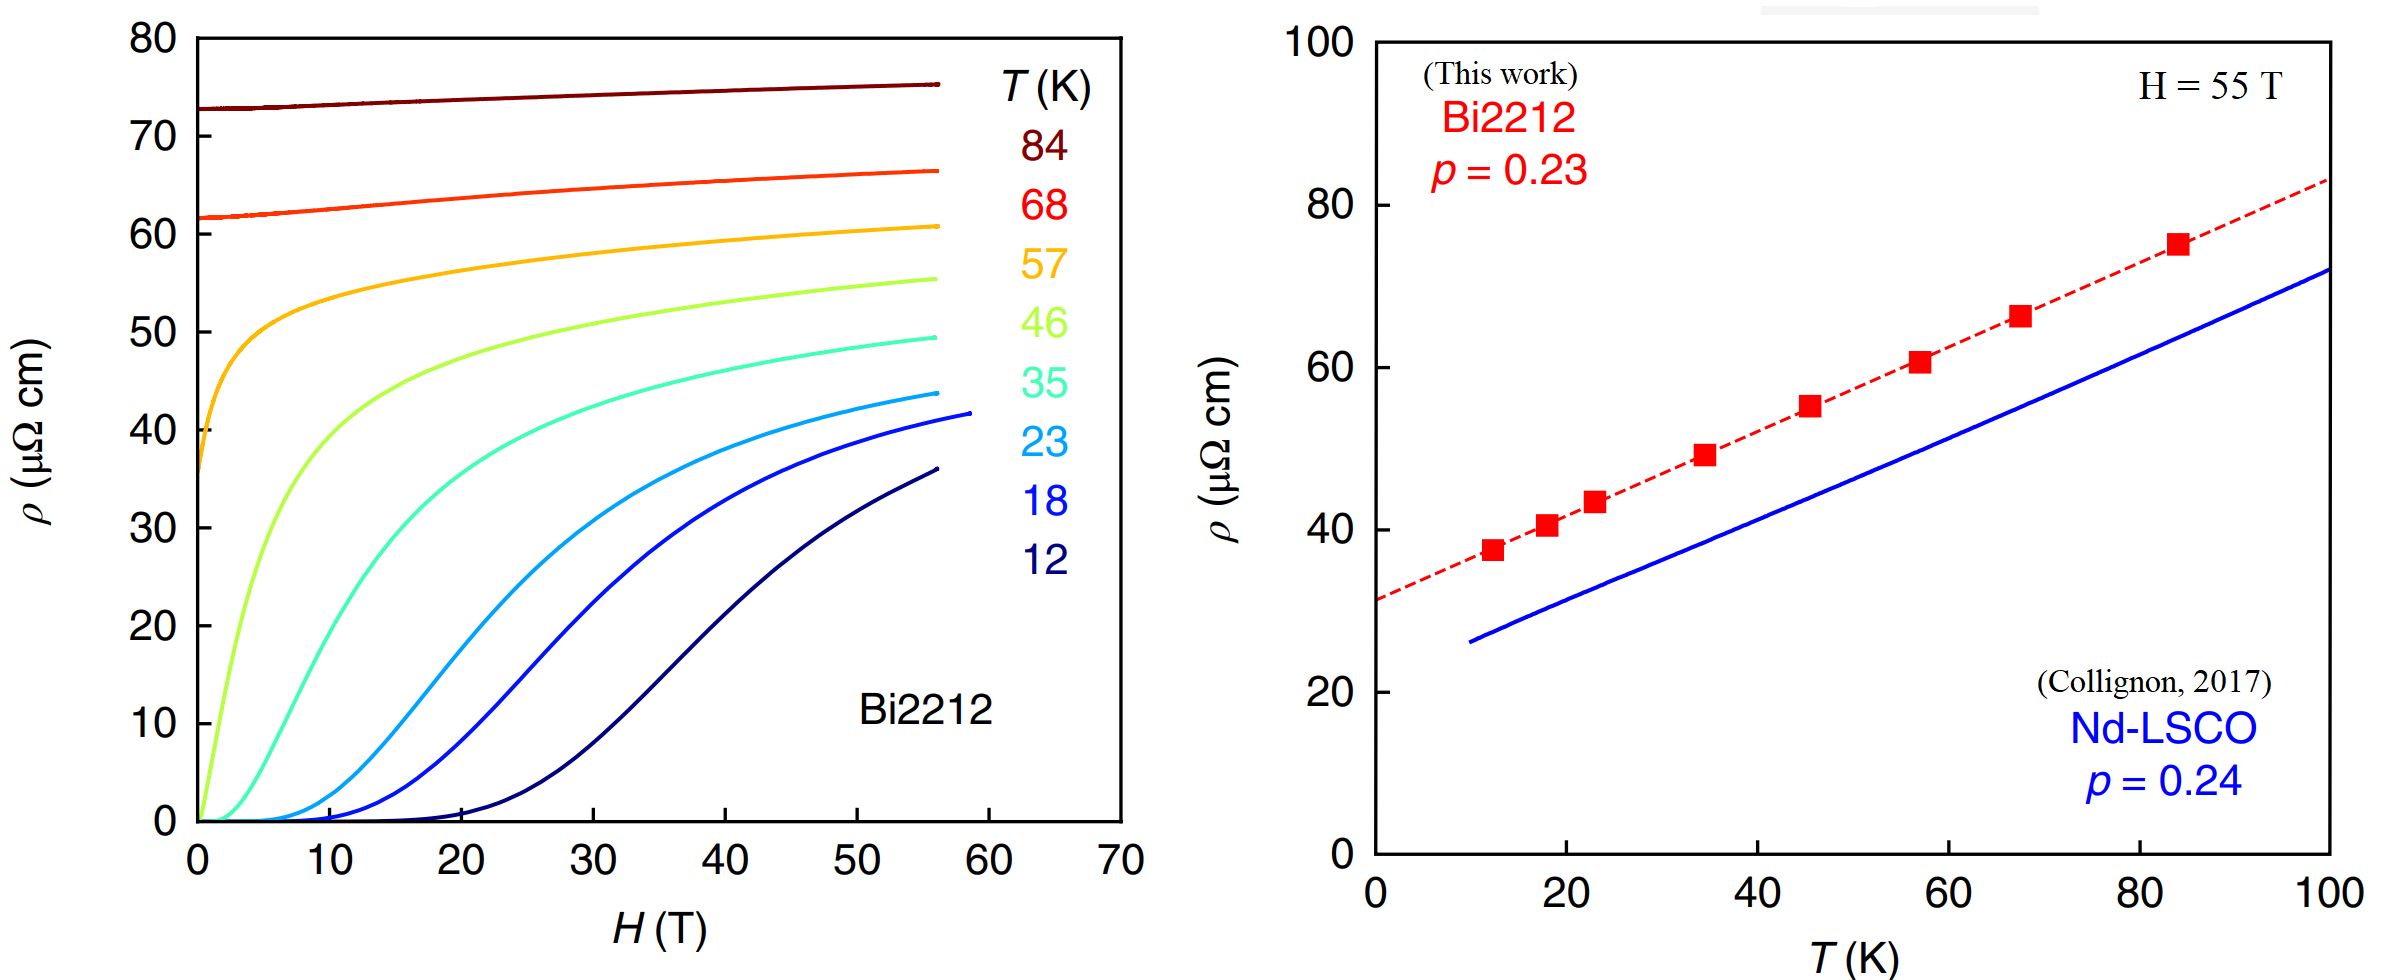
\includegraphics[width=4.3in]{figs/rho_bscco_2.png}
\end{figure}
\begin{itemize}
\item The slope per CuO$_2$ plane is $A = 8.0 \pm 0.9~\rm{\Omega K^{-1}}$
\item This is the same as Nd-LSCO at $p = 0.24$, where $A = 7.4 \pm 0.8~\rm{\Omega K^{-1}}$
\end{itemize}
Conclusion: $T$-linear resistivity doesn't change with the Fermi surface and $T_\text{c}$
\end{frame}

\begin{frame}{Resistivity of PCCO at $p = 0.17$}
\begin{figure}
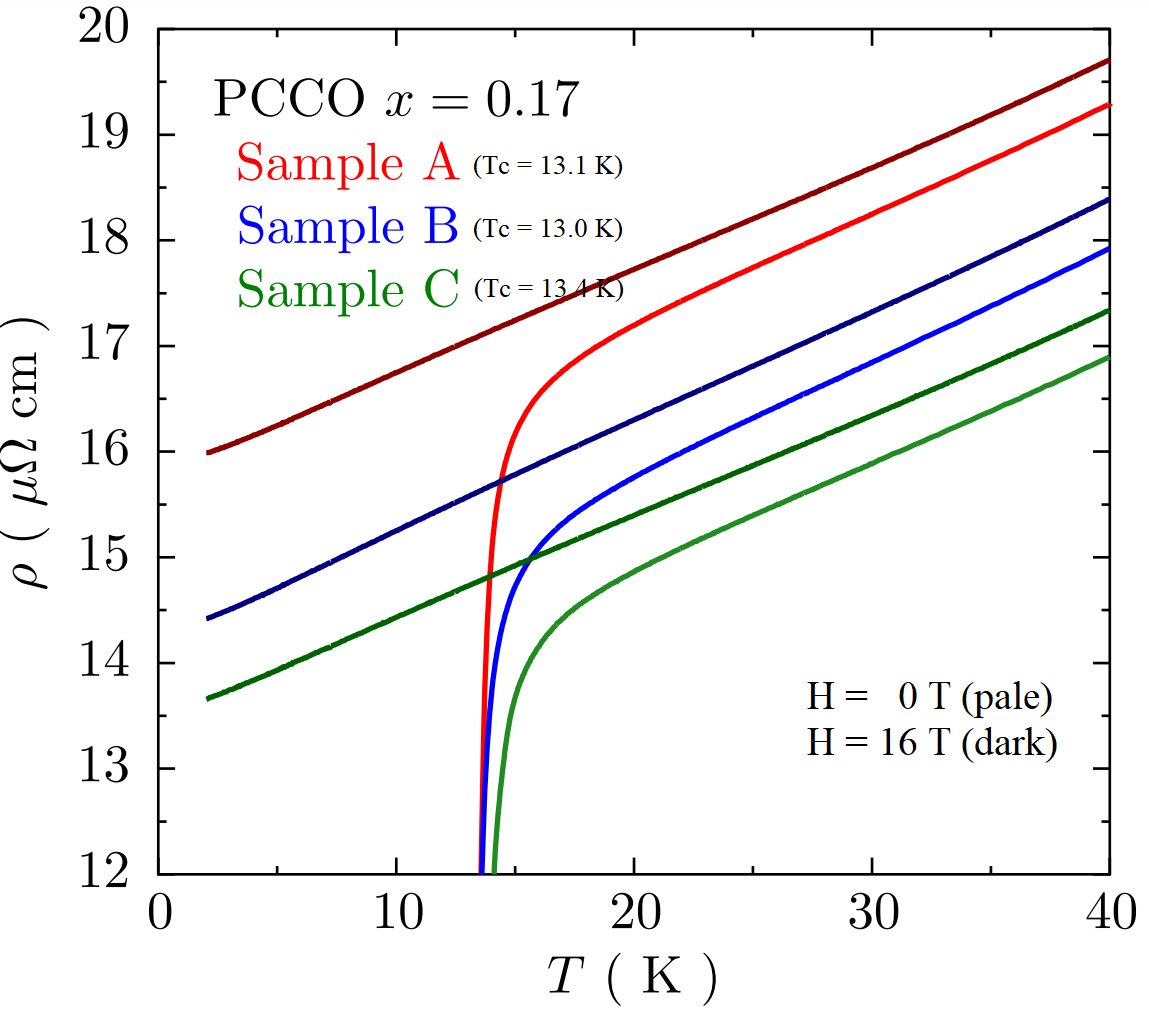
\includegraphics[width=2.8in]{figs/rho_pcco_2.png}
\end{figure}
\begin{itemize}
\item The slope per CuO$_2$ plane is $A = 1.7 \pm 0.3~\rm{\Omega K^{-1}}$ (about 4 times smaller than the hold-doped case)
\end{itemize}
\end{frame}

\begin{frame}{Slope per CuO$_2$ plane ($A$) vs. doping ($p$)}
\begin{figure}
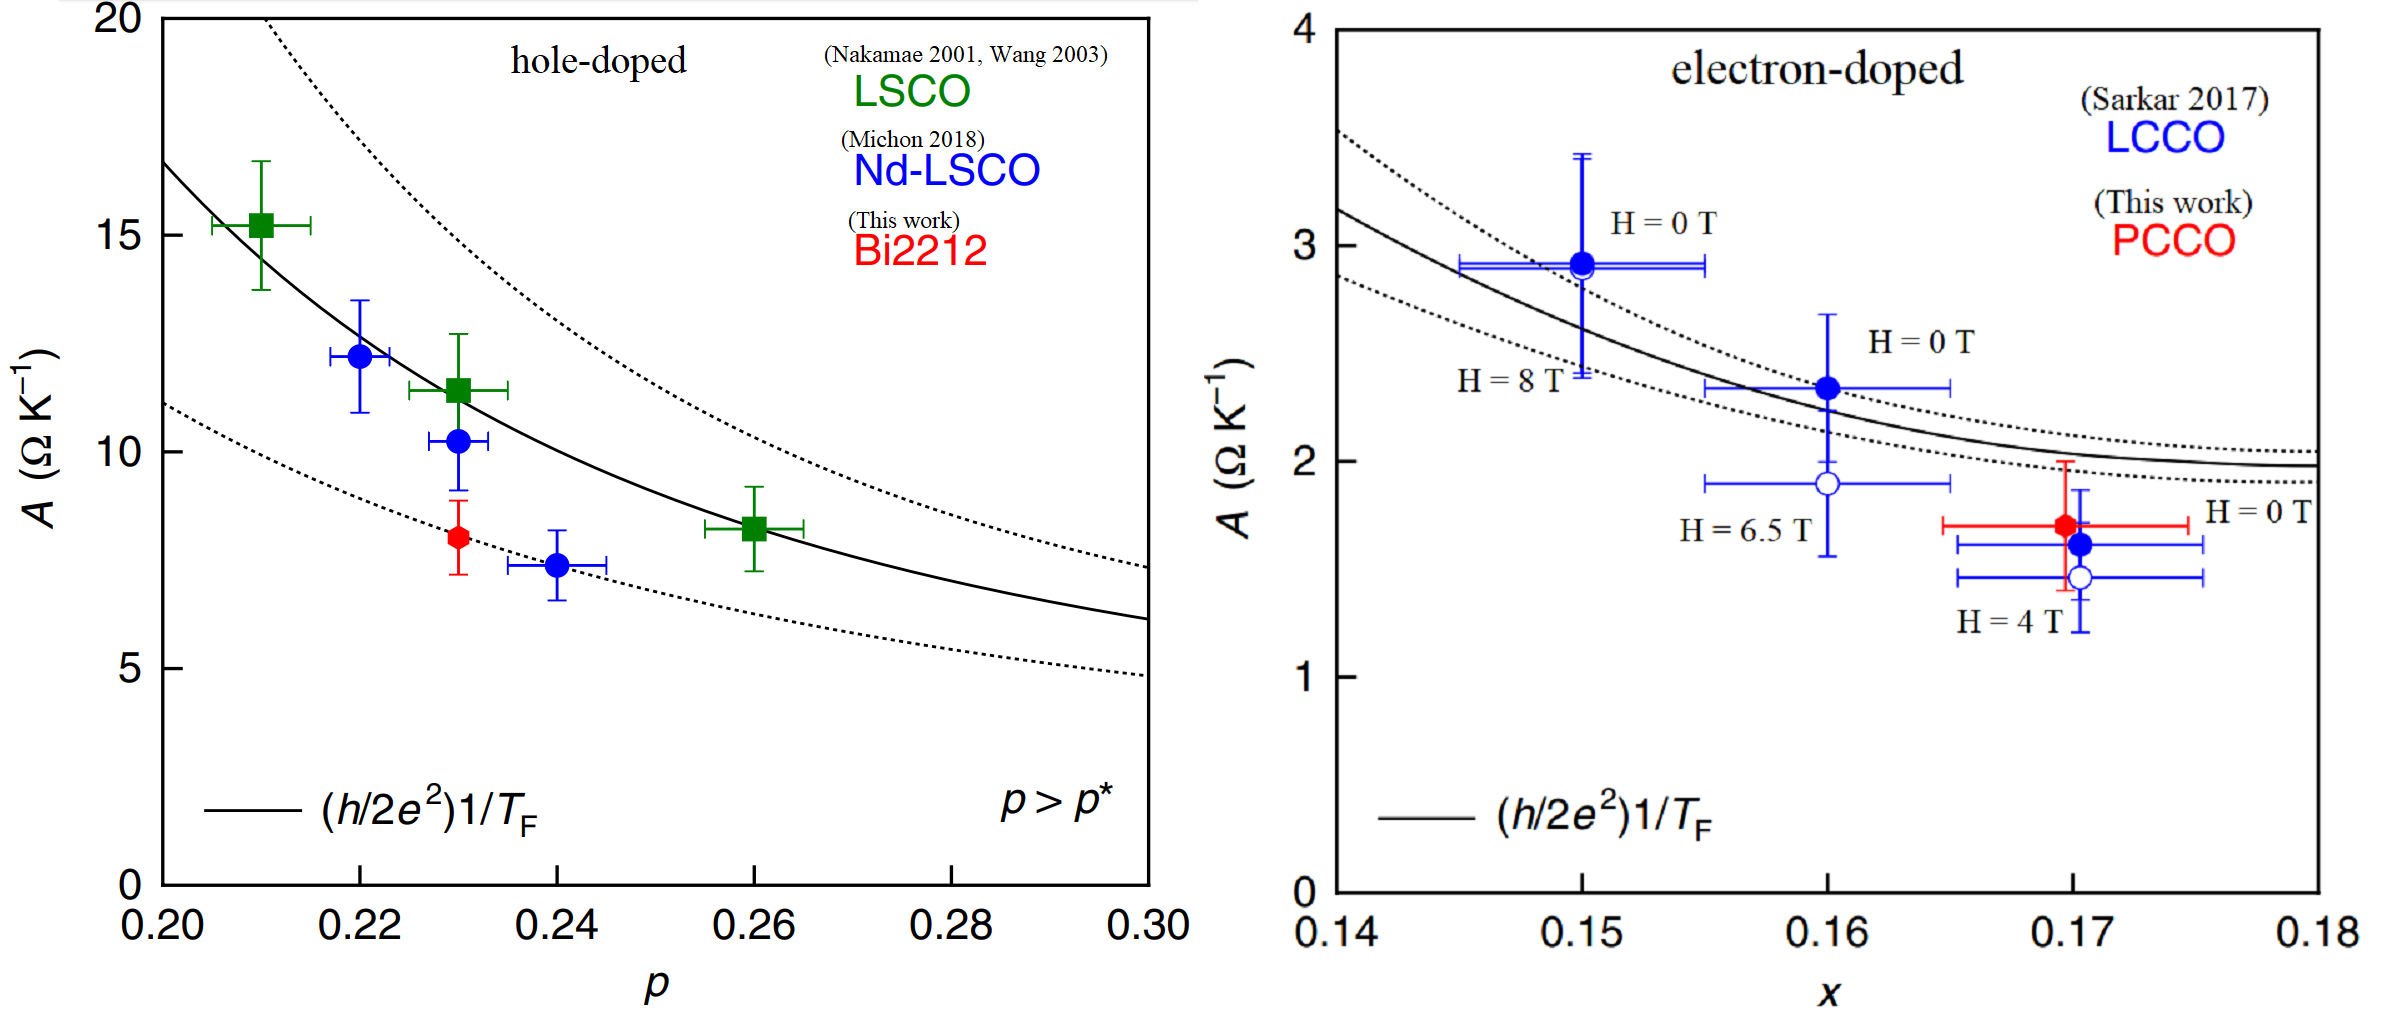
\includegraphics[width=5in]{figs/A_vs_p_both.png}
\end{figure}
Conclusion: $A$ increases as $p$ decreases in hole-doped and electron-doped cuprates
\end{frame}
% Not sure if it is justified to fit the data from different materials

\begin{frame}{How to calculate the solid lines from the previous slide}
\begin{itemize}
\item Several metals exhibit $T$-linear $\rho$ when $\hbar/\tau = k_\text{B}T$ (the Plankian limit) (Bruin 2013)
\item So, we write $\hbar/\tau = \alpha k_\text{B}T$, where $\alpha$ measures how close to the Plankian limit
\item For isotropic Fermi surface, $\rho = (m^{\ast}/ne^2)(1/\tau)$ (the Drude formula)
\item Thus, when $\rho(T) = \rho_0 + [\text{slope}] T$, $\text{slope} = \alpha (m^{\ast}/n)(k_\text{B}/e^2 h)$
\item The slope per CuO$_2$ plane is
\begin{align}
A &= \alpha \left(\frac{h}{2e^2}\right) \frac{1}{T_\text{F}},
\end{align}
where $T_\text{F} = (\pi \hbar^2/k_\text{B}) (nd/m^{\ast})$, $n = (1-x)/(a^2 d)$, and the effective mass $m^{\ast}$ is measured from the specific heat coefficient $\gamma$:
\begin{align}
\gamma &= (\pi N_{\text{A}} k_\text{B}^2 / 3 \hbar^2) a^2 m^{\ast}.
\end{align}
\item $\alpha$ can be calculated from $A$ and other measurable variables
\end{itemize}
\end{frame}
% alpha is the ratio between experimental and predicted values?

\begin{frame}{$\alpha$ in various materials}
\begin{table}
\begin{tabular}{llll}
Material & Doping & $A~(\rm{\Omega K^{-1}})$ & $\alpha$ \\
\hline
BSCCO & $p = 0.23$ & $8.0 \pm 0.9$ & $1.1 \pm 0.3$ \\
BSCCO & $p = 0.40$ & $8.0 \pm 2.0$ & $1.0 \pm 0.4$ \\
LSCO & $p = 0.26$ & $8.2 \pm 1.0$ & $0.9 \pm 0.3$ \\
Nd-LSCO & $p = 0.24$ & $7.4 \pm 0.8$ & $0.7 \pm 0.4$ \\
PCCO & $x = 0.17$ & $1.7 \pm 0.3$ & $0.8 \pm 0.2$ \\
LCCO & $x = 0.15$ & $3.0 \pm 0.5$ & $1.2 \pm 0.3$ \\
TMTSF & ? & $2.8 \pm 0.3$ & $1.0 \pm 0.3$ \\
\end{tabular}
\end{table}
Conclusion: $\alpha = 1.0$ for all cases within error bars
\end{frame}

\begin{frame}{Implications}
\begin{itemize}
\item Organic superconductors (TMTSF), heavy-fermion metals and pnictides share the same scattering rate and $T$-linear resistivity feature
\end{itemize}
\end{frame}

\begin{frame}{Conclusion}
\begin{itemize}
\item
\end{itemize}
\end{frame}

\end{document}
